% Document class report-template accepts either: project-plan or final-report option
\documentclass[project-plan]{report-template}

% Packages I want to use in my report.
\usepackage{graphicx}
\usepackage{amsmath}
\usepackage{blindtext}

% Directory where I save my figures.
\graphicspath{{./figures/}}

% Metadata used for the title page.
\university{Imperial College London}
\department{Department of Earth Science and Engineering}
\course{MSc in Applied Computational Science and Engineering}
\title{Forecasting induced seismicity in Oklahoma}
\author{Zhiyong Liu}
\email{zl1220@ic.ac.uk}
\githubusername{acse-liuzyon}
\supervisors{Dr. Stephen P. Hicks}
\repository{https://github.com/acse-2020/acse2020-acse9-projectplan-liuzyon}

\begin{document}

\maketitlepage  % generate title page
\githubrepo  % GitHub repository

% Abstract
\section*{Abstract}
\blindtext  % outputs some dummy text
\newpage

% Introduction section
\section{Introduction}
It is well known that humans can cause earthquakes through fluid injection and extraction. Ellsworth stated the understanding of the causes and mechanics of human-induced earthquakes. It includes wastewater injection, emerging oil and gas recovery technologies, and other indirect induced activities,
including deep fluid injection \citep{ellsworth2013injection}.
Such cases of induced seismicity have been recorded and proven in Oklahoma, where seismicity has been increased dramatically since 2010 \citep{ellsworth2013injection}.
In cases like Oklahoma, because the rate of earthquakes was very low before high-rate wastewater injection, it is relatively easy to determine the fundamental causes of induced seismicity.
Therefore, due to the low background stress in intraplate regions, the human triggering signatures are clearly identifiable.
However, in tectonically-active areas, it is more challenging to distinfuish between natural and triggered seismicity.
In tectonically active regions in the US, such as California, although oil and gas extraction has taken place for many decades, only a handful of studies have been published with a focus on these areas \citep{Hough2017WasTM}. 
In these areas, Big-data and statistical approaches will be crucial in separating natural causes from potential human triggering factors.
Hincks et al. developed a Bayesian network to for quantitative evaulation of correlations between well operational parameters, geological formation, and seismicity.
The injection depth relative to crystalline basement was found to be the most significant parameter for seismic moment release \citep{hincks2018oklahoma}.


Wozniakowska and Eaton performed a machine learning estimation of the seismogenic activation potential for each well using logistic regression and found that the injection depth influence greatly the seismogenic activation potential \citep{wozniakowska2020machine}.
Norbeck and Rubinstein genreated a model based on fluid flow and seismic physics, which associate the past injection trends with the seismicity patterns \citep{norbeck2018hydromechanical}.

The correlations of induced earthquakes with fluid extraction and injection are well established. 
Some physics models are also developed in previous research for earthquake prediction.
However, these researches do not explain why seismicity does not always occured close to an injection well.
Also, these studies did not develop a statistical model or a machine-learning model to predict earthquakes based on well documented data (such recorded data in Oklahoma)

% Another section
\section{My section}
In this work, we implemented code for computing the position of a particle in vertical motion as shown in Fig.~\ref{fig:experiment}. The position $y(t)$ at time $t$ we compute using:

\begin{equation}
    \label{eq:vertical-position}
    y(t) = v_{0}t - \frac{1}{2}gt^{2},
\end{equation}

where $v_{0}$ is the initial velocity, and $g$ is the acceleration due to the Earth's gravity.

\begin{figure}
    \begin{center}
        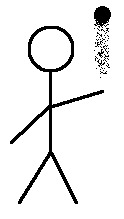
\includegraphics[width=0.2\textwidth]{experiment.jpg}
    \end{center}
    \caption{\label{fig:experiment} Particle in vertical motion.}
\end{figure}

The Python code we implemented for computing $y(t)$ is:

\begin{lstlisting}[language=Python]
def position(t, v0=0, g=9.81):
    """My function."""
    return v0*t - 0.5*g*t**2
\end{lstlisting}

We made our computational workflows reproducible by employing all benefits of the Jupyter environment~\citep{Beg2021}.

\section*{Conclusions}
\blindtext[2]

% References
\bibliographystyle{agsm}
\bibliography{references.bib}  % BibTeX references are saved in references.bib

\end{document}          

